% CVPR 2024 Paper Template; see https://github.com/cvpr-org/author-kit

\documentclass[10pt,twocolumn,letterpaper]{article}

%%%%%%%%% PAPER TYPE  - PLEASE UPDATE FOR FINAL VERSION
\usepackage{cvpr}              % To produce the CAMERA-READY version
% \usepackage[review]{cvpr}      % To produce the REVIEW version
% \usepackage[pagenumbers]{cvpr} % To force page numbers, e.g. for an arXiv version

% Import additional packages in the preamble file, before hyperref
%
% --- inline annotations
%
\usepackage[dvipsnames]{xcolor}
\newcommand{\red}[1]{{\color{red}#1}}
\newcommand{\todo}[1]{{\color{red}#1}}
\newcommand{\TODO}[1]{\textbf{\color{red}[TODO: #1]}}
% --- disable by uncommenting  
% \renewcommand{\TODO}[1]{}
% \renewcommand{\todo}[1]{#1}



% It is strongly recommended to use hyperref, especially for the review version.
% hyperref with option pagebackref eases the reviewers' job.
% Please disable hyperref *only* if you encounter grave issues, 
% e.g. with the file validation for the camera-ready version.
%
% If you comment hyperref and then uncomment it, you should delete *.aux before re-running LaTeX.
% (Or just hit 'q' on the first LaTeX run, let it finish, and you should be clear).
\definecolor{cvprblue}{rgb}{0.21,0.49,0.74}
\usepackage[pagebackref,breaklinks,colorlinks,citecolor=cvprblue]{hyperref}

%%%%%%%%% PAPER ID  - PLEASE UPDATE
\def\paperID{*****} % *** Enter the Paper ID here
\def\confName{CVPR}
\def\confYear{2024}

%%%%%%%%% TITLE - PLEASE UPDATE
\title{Toy Models of Superposition Review}

%%%%%%%%% AUTHORS - PLEASE UPDATE
\author{Sean Murphy\\
Monash University\\
Melbourne, Australia\\
{\tt\small smur0055@student.monash.edu}
% For a paper whose authors are all at the same institution,
% omit the following lines up until the closing ``}''.
% Additional authors and addresses can be added with ``\and'',
% just like the second author.
% To save space, use either the email address or home page, not both
\and
Leo Qiao\\
Monash University\\
Melbourne, Australia\\
{\tt\small lqia0021@student.monash.edu}
}

\begin{document}
\maketitle
\section{Review}
\label{sec:review}

The \textit{Toy Models of Superposition} paper \cite{elhage2022toy} published in 2022 by researchers from Anthropic and Harvard University, investigates "superposition", a phenomenon where neural networks represent more features than they have available dimensions.
They define a \textit{feature} as an interpretable property of the input that neurons respond to.
The paper focuses on how neural networks overcome their limited dimensions through the use of polysemantic neurons, which represent multiple features at once.

The authors use a toy model to demonstrate superposition by training it to project five features onto only two dimensions, then attempting to recover the original features.
One key finding is that the sparsity of a feature—how rarely it occurs—is a primary factor in determining whether it is represented in superposition. For instance, when features are not sparse, only the two most important ones are represented in dedicated orthogonal dimensions.
However, as sparsity increases, the model begins to encode all five features in superposition, arranging them geometrically in a pentagon-like structure within the two-dimensional space.
This results in interference between the features, where one's presence also activates other unrelated neurons.

The middle sections of the paper provide a mathematical explanation for why superposition occurs, whilst also exploring the specific "phases" of superposition that can occur under different conditions.
The paper concludes by discussing how "solving superposition" could lead to more interpretable and safer AI models.
They suggest that a key step in achieving this would be the ability to identify and enumerate all features in a model—what they refer to as the fundamental units of a neural network.
With such an understanding, one could potentially produce a universal quantifier over these features, which could be used to fully explain model behaviour and thus enable confidence that models would not simply avoid, but perhaps be entirely incapable of unethical behaviours like deception.
The authors propose that this might be achieved either by designing models that avoid superposition entirely or by finding an overcomplete basis that disentangles the superimposed features, motivating future research directions.

%-------------------------------------------------------------------------

\subsection{Significance}

The concept of superposition, as explored in this paper, holds significant implications for both our theoretical understanding of neural networks and practical advancements in mechanistic interpretability and AI safety.
It provides an entirely new perspective on the fundamental units of neural networks by showing how polysemantic neurons can be broken down into multiple features.
With over 200 citations in just 2 years, this paper has fueled a lot of modern day mechanistic interpretability research.

\subsection{Relevance in the Deep Learning Era}

In the current deep learning era, where advancements in model capabilities are positively correlated with model complexity, continuing to iterate this way only creates bigger, and bigger black boxes.
The insights this paper presents regarding the superposition phenomenon suggest alternate directions that would allow us to better understand these black boxes by "solving superposition".

Additionally, this paper shows the importance of model architecture, illuminating the tradeoff between efficiency brought about by smaller model sizes, and the interference caused by the superpositional feature representations that it necessitates.
As our understanding of model features matures, there is potential for model architecture hyperparams to be more analytically selected given information about the data, such as feature sparsity.
If we are able to obtain universal quantifiers over features as the paper suggests, we may even see a shift in the deep learning era where engineers can build or modify parts of these networks manually, having the ability to dictate the inclusion of specific features, and change the semanticity of neurons at will.

\section{Superposition as a Cause of Hallucinations}
\label{sec:superposition_as_a_cause_of_hallucinations}

A key question from the paper was whether interference from superposition causes hallucinations in large language models.
To test this, we trained a classifier on high-sparsity data, inducing superposition, and evaluated it on low-sparsity data.

\subsection{Dataset}
We used a dataset with five features, represented by English affixes: \textit{un-}, \textit{re-}, \textit{-able}, \textit{-ful}, \textit{-ness}, although any set of affixes could work.
Two datasets were generated: one with words containing a single affix (pure words) and another with words containing multiple affixes (dual words, e.g., \textit{unreliable}).
The pure dataset was split into training and test sets, while the dual dataset was reserved for evaluation.

\subsection{Model}
We trained a model with an embedding layer, a convolutional layer, a hidden layer, and ReLU activation.
The hidden layer had only two neurons, forcing it to use superposition to encode all five features.

\subsection{Results}
Using the \href{https://colab.research.google.com/github/anthropics/toy-models-of-superposition/blob/main/toy_models.ipynb}{toy model framework}, we visualized the five features in the hidden layer.
\begin{figure}[h]
	\centering
	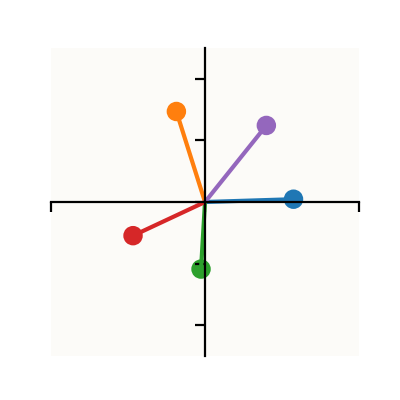
\includegraphics[width=0.3\linewidth]{figures/hallucinations_hidden_layer.png}
	\caption{Representation of the five features in the hidden layer.}
	\label{fig:hidden_layer_representation}
\end{figure}
Figure \ref{fig:hidden_layer_representation} shows the model all features, though it didn't form the pentagon-like structure noted in the paper.
Table \ref{tab:hallucinations_results} shows the results for the test set and the dual dataset.
\begin{table}[h]
	\centering
	\begin{tabular}{lc}
		\toprule
		\textbf{Dataset} & \textbf{Accuracy} \\
		\midrule
		Test set         & 0.9772            \\
		Dual dataset     & 0.9581            \\
		\bottomrule
	\end{tabular}
	\caption{Model evaluation on the test set and the dual dataset.}
	\label{tab:hallucinations_results}
\end{table}
The model performed well on the test set, but accuracy dropped on the dual dataset, even though each dual word had twice the correct labels.
This suggests that when features are less sparse than in training, the additive interference from superposition may cause misinterpretations, contributing to hallucinations in large language models.

\section{Inhibiting Superpositions with Activations}
\label{sec:act_fns}
The paper presents the activation function as a key in enabling the formation of superpositions due to their ability to 
filter out interference. As such, we demonstrate that modifying the activation can effectively control the model's usage of
superpositions. 
\newline
We propose ExReLU, a modified version of ReLU with a cut-off threshold of $t \in \mathbb{R}$, instead of $0$. By setting $t < 0$, its filtering effect for negative interference is weakened, thus
increasing the cost for the model to adopt superpositional representations.
\[
\text{ExReLU}(x) =
    \begin{cases}
        x & \text{if } x \geq t\\
        0 & \text{if } x < t
    \end{cases}
\] 

\subsection{Model}
We trained two sets of models, each with hidden layers of two neurons on a dataset with five features whilst varying the feature
sparsity. The first set used the normal ReLU activation, while the second used ExReLU with $t=-0.25$

\subsection{Results}
\begin{figure}[h]
	\centering
	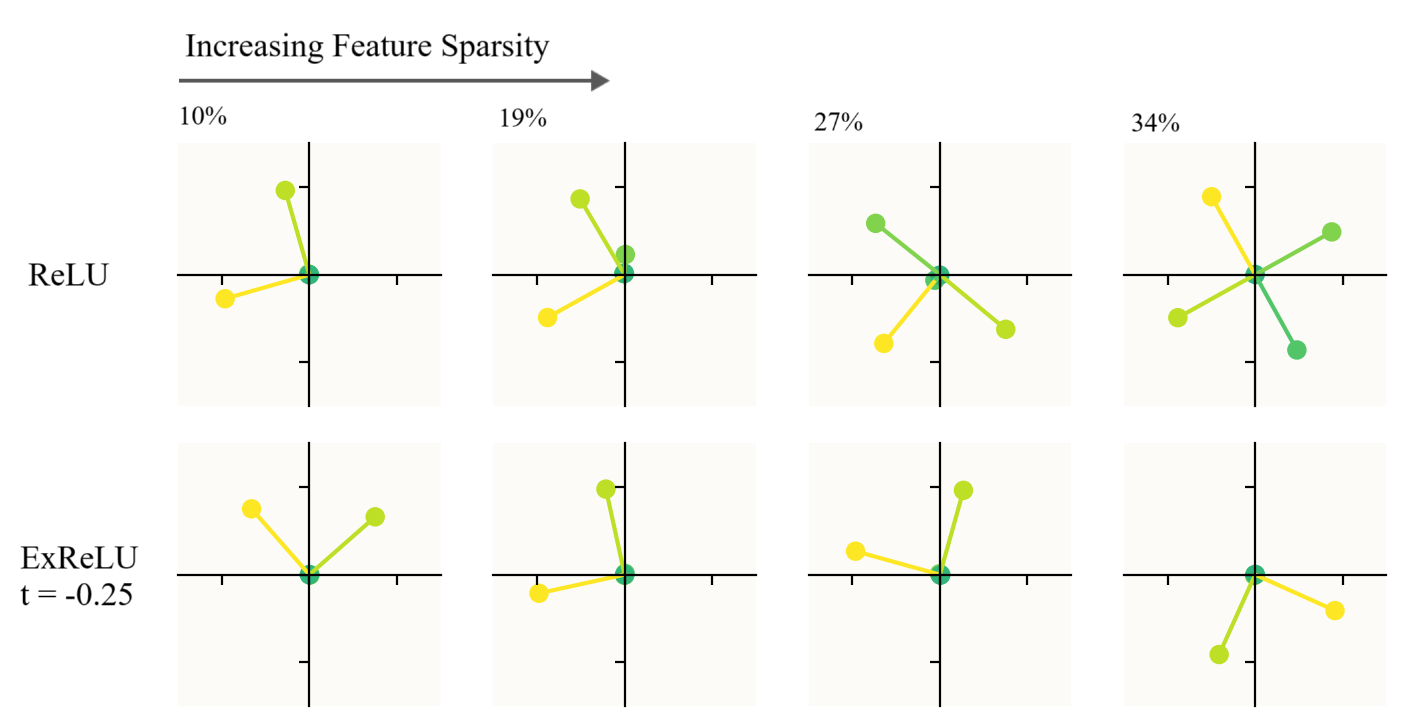
\includegraphics[width=1\linewidth]{figures/acts_diagram.png}
	\caption{Comparison of feature embeddings by the two model sets.}
	\label{fig:acts_diagram}
\end{figure}
Using the \href{https://colab.research.google.com/github/anthropics/toy-models-of-superposition/blob/main/toy_models.ipynb}{toy model framework} to visualize the hidden layer's representation of the features:
Figure \ref{fig:acts_diagram} shows that ExReLU has successfully suppressed the model's usage of superpositions in this instance.
As such, it seems that the development of new activation functions akin to ExRELU may be key to 'solving superposition' and controlling how models 
use their available dimensions as mentioned in the paper.
{
	\small
	\bibliographystyle{ieeenat_fullname}
	\bibliography{main}
}

% WARNING: do not forget to delete the supplementary pages from your submission 
% \clearpage
\setcounter{page}{1}
\maketitlesupplementary


\section{Rationale}
\label{sec:rationale}
% 
Having the supplementary compiled together with the main paper means that:
% 
\begin{itemize}
\item The supplementary can back-reference sections of the main paper, for example, we can refer to \cref{sec:intro};
\item The main paper can forward reference sub-sections within the supplementary explicitly (e.g. referring to a particular experiment); 
\item When submitted to arXiv, the supplementary will already included at the end of the paper.
\end{itemize}
% 
To split the supplementary pages from the main paper, you can use \href{https://support.apple.com/en-ca/guide/preview/prvw11793/mac#:~:text=Delete%20a%20page%20from%20a,or%20choose%20Edit%20%3E%20Delete).}{Preview (on macOS)}, \href{https://www.adobe.com/acrobat/how-to/delete-pages-from-pdf.html#:~:text=Choose%20%E2%80%9CTools%E2%80%9D%20%3E%20%E2%80%9COrganize,or%20pages%20from%20the%20file.}{Adobe Acrobat} (on all OSs), as well as \href{https://superuser.com/questions/517986/is-it-possible-to-delete-some-pages-of-a-pdf-document}{command line tools}.

\end{document}
